%% Define title of slide deck

\newcommand\CourseTopic{Numerical Analysis}
\newcommand\CourseTopicShort{Numerical Analysis}
\newcommand\CourseNumber{4}

\newcommand\CourseDate{\today}
\newcommand\CourseInstitute{ETH Zurich}
\newcommand\CourseAbbreviation{OR}
\newcommand\CourseTitle{Operations Research in R}
\newcommand\CourseAuthor{Stefan Feuerriegel}

\newcommand{\CourseQuiz}{Visit webpage with course quiz.}
\newif\ifQuizSolution\QuizSolutionfalse

\PassOptionsToPackage{table,dvipsnames}{xcolor}
\documentclass[%
  final,
  11pt, 
  show notes, % enables Notes
  t, % Place text of slides at the (vertical) top of the slides
  fleqn, % equations are centered
]{beamer} 

\usepackage{booktabs}

\newcommand\const{\mathsf{const.}}
\newcommand\rp{^{-1}}
\newcommand\rps{^{-2}}
\newcommand\rpc{^{-3}}

\newcommand\transpose{^T} %{^\top}
\newcommand\rptranspose{^{-T}} %^{^{-\top}}
\newcommand\pseudoinverse{^{+}}

\newcommand\define{:=} % :=, \ensuremath{\mathrel{\stackrel{\mathsf{def}}{=}}}
\newcommand\ldefine{=:}
\newcommand{\setsep}{\, | \,}

\newcommand{\correspond}{\mathrel{\widehat{=}}}

\newcommand{\norm}[1]{\left\Vert #1 \right\Vert}
\newcommand{\floor}[1]{\left\lfloor #1 \right\rfloor}
\newcommand{\ceil}[1]{\left\lceil #1 \right\rceil}

\newcommand{\vecval}[1]{\bm{#1}}
\newcommand{\matval}[1]{#1}

\newcommand{\sspace}{\quad}
\newcommand{\wspace}{\qquad}

\newcommand{\sand}{\sspace\text{and}\sspace}
\newcommand{\wand}{\wspace\text{and}\wspace}
\newcommand{\for}{\text{for }}

\newcommand{\R}{\mathbb{R}}
\newcommand{\N}{\mathbb{N}}

\newcommand{\unitvec}[2]{{\vecval{u}_{#1}}}
\newcommand{\identitymat}[1]{\matval{\mathup{I}}_{#1,#1}}
\newcommand{\permutemat}{\matval{\Pi}}
\newcommand{\zerovec}[1]{\vecval{0}_{#1}}
\newcommand{\zeromat}[2]{\matval{0}_{#1,#2}}

\newcommand{\fulfill}{\stackrel{!}{=}}
\newcommand{\inlineortho}{\bot}
\newcommand{\ortho}{\,\, \inlineortho \,\,}
\newcommand{\iszero}[1]{\underbrace{#1}_{=0}}

\newcommand{\vecsize}[1]{\in\R^{#1}}
\newcommand{\matsize}[2]{\in\R^{#1 \times #2}}

\newcommand{\concatmat}[1]{\Concat{#1}}
\newcommand{\concatvec}[1]{\left[#1\right]}
\newcommand{\concatmatsep}{\, | \,}
%\newcommand{\lincomb}[1]{\left\langle #1 \right\rangle}
\newcommand{\lincomb}[1]{\linearspan{#1}}
%\newcommand{\vecprod}[2]{\left( #1, #2 \right)}
\newcommand{\vecprod}[2]{\left\langle #1, #2 \right\rangle}

\newcommand{\abs}[1]{\left\lvert #1 \right\rvert}
\newcommand{\sign}[1]{\mathup{sign}\left( #1 \right)}
%\newcommand{\ssign}{\mathsf{sign}}
\newcommand{\diag}{\operatorname{diag}}
%\renewcommand\Re[1][]{\mathsf{Re}\,#1}
%\renewcommand\Im[1][]{\mathsf{Im}\,#1}

\newcommand{\vvector}[2]{\left[\begin{array}{c} #1 \\ #2 \end{array} \right]}
\newcommand{\vvvector}[3]{\left[\begin{array}{c} #1 \\ #2 \\ #3 \end{array} \right]}

\newcommand{\intervaloo}[2]{\left(#1,#2\right)}
\newcommand{\intervaloc}[2]{\left(#1,#2\right]}
\newcommand{\intervalco}[2]{\left[#1,#2\right)}
\newcommand{\intervalcc}[2]{\left[#1,#2\right]}

\newenvironment{mmatrix}{\begin{bmatrix}}{\end{bmatrix}}

\newcommand{\Oh}[1]{\mathsf{O}\left(#1\right)}

\newcommand{\e}[1]{\mathup{e}^{#1}}

\newcommand{\dd}{\mathop{}\!\mathsf{d}}
\newcommand{\Laplace}{\Updelta}

\newcommand\op[1]{{\hat{\mathsf{#1}}}}  % Operator

\newcommand\imaginary{\mathup{i}}

% use together with long limits in \sum, \prod, etc
% from mathmode, p. 63
  \def\clap#1{\hbox to 0pt{\hss#1\hss}}
  \def\mathclap{\mathpalette\mathclapinternal}
  \def\mathclapinternal#1#2{%
    \clap{$\mathsurround=0pt#1{#2}$}
  }

\newcommand\ie{i.\,e.\xspace}
\newcommand\eg{e.\,g.\xspace}
\newcommand\etc{etc.\xspace}
\newcommand\cf{cf.\xspace}

%% from: http://tex.stackexchange.com/questions/2441/how-to-add-a-forced-line-break-inside-a-table-cell
\newcommand{\mcell}[2][c]{%
  \begin{tabular}[c]{@{}#1@{}}#2\end{tabular}}
\newcommand{\mcellt}[2][c]{%
  \begin{tabular}[t]{@{}#1@{}}#2\end{tabular}}

\newcommand{\stackedcell}[2][c]{%
  \begin{tabular}[#1]{@{}c@{}}#2\end{tabular}}

<<setup, include=FALSE>>=
# change default language to display error messages in English
Sys.setenv(LANGUAGE = "en")

# smaller font size for chunks
library(knitr)
opts_chunk$set(size = "footnotesize", fig.width = 3, fig.height = 3)
@

\begin{document}

  \begin{frame}%[plain]
  \titlepage
\end{frame}
  
\begin{frame}
  \frametitle{Today's Lecture}
\vfill
\begin{block}{Objectives}
\begin{enumerate}
\item Understanding how computers store and handle numbers
\item Repeating basic operations in linear algebra and their use in R
\item Recapitulating the concept of derivatives and the Taylor approximation
\item Formulating necessary and sufficient conditions for optimality
\end{enumerate}
\end{block}
\vfill
\end{frame}
  
  % \section[Contents]{}

\begin{frame}<beamer>%[allowframebreaks]
  \frametitle{Outline}
  \tableofcontents[%
%     currentsection, % causes all sections but the current to be shown in a semi-transparent way.
%     currentsubsection, % causes all subsections but the current subsection in the current section to ...
%     hideallsubsections, % causes all subsections to be hidden.
%     hideothersubsections, % causes the subsections of sections other than the current one to be hidden.
%     part=, % part number causes the table of contents of part part number to be shown
%    pausesections, % causes a \pause command to be issued before each section. This is useful if you
%     pausesubsections, %  causes a \pause command to be issued before each subsection.
%     sections={ overlay specification },
%      sectionstyle=show/shaded,
      subsectionstyle=hide
  ]
\end{frame}

\section{Number Representations}

\begin{frame}
  \frametitle{Positional Notation}
\begin{itemize}
\item Method of \emph{representing numbers}
\item Same symbol for different orders of magnitude ($\neq$ Roman numerals)
\item \emph{Format} is $d_n d_{n-1} \ldots d_2 d_1 =  d_n \cdot b^{n-1} + d_{n-1} \cdot b^{n-2} + \ldots + d_2 \cdot b + d_1$ \\
with\\
\qquad
\begin{tabular}{ll}
$b$ & \emph{base} of the number \\
$n$ & number of digits \\
$d$ & digit in the $i$-th position of the number\\
\end{tabular} 
\item Example: 752 is $7_3 \cdot 10^2 + 5_2 \cdot 10 + 2_1$
\end{itemize}
\end{frame}

\begin{frame}
  \frametitle{Base Conversions}
\begin{itemize}
\item Numbers can be \emph{converted between bases}
\begin{itemize} 
\item Base 10 is default
\item \emph{Binary system} with base 2 common for computers
\end{itemize}
\item Example: 752 in base 10 equals 1\,011\,110\,000 in base 2
\vspace*{0.3cm}
\item \emph{Conversion from base $b$ into base 10} via
\begin{equation*}
d_n \cdot b^{n-1} + d_{n-1} \cdot b^{n-2} + \ldots + d_2 \cdot b + d_1
\end{equation*}
\item Example: $101\,101\,011$ in base 2 
\end{itemize}
\begin{align*}
& 1 \cdot 2^8 + 0 \cdot 2^7 + 1 \cdot 2^6 + 1 \cdot 2^5 + 0 \cdot 2^4 + 1 \cdot 2^3 + 0 \cdot 2^2 + 1 \cdot 2^1 + 1 \\
= & 1 \cdot 256 + 0 \cdot 128 + 1 \cdot 64 + 1 \cdot 32 + 0 \cdot 16 + 1 \cdot 8 + 0 \cdot 4 + 1 \cdot 2 + 1 \\
= & 363 \text{ in base 10}
\end{align*}
\end{frame}

\begin{frame}
  \frametitle{Base Conversions}
\begin{exampleblock}{Question}
\begin{itemize}
\item Convert the number 10\,011\,010 from base 2 into base 10
\begin{itemize}
\item 262
\item 138
\item 154
\end{itemize}
\item \CourseQuiz
\end{itemize}
\end{exampleblock}
%{\footnotesize $\rightarrow$ $1 \cdot 128 + 0 \cdot 64 + 0 \cdot 32 + 1 \cdot 16 + 1 \cdot 8 + 0 \cdot 4 + 1 \cdot 2 + 0 = 154$
%}
\pause
\vspace*{0.4cm}
\begin{exampleblock}{Question}
\begin{itemize}
\item Convert the number 723 from base 10 into base 2
\begin{itemize}
\item 111\,010\,011
\item 10\,011\,010\,011
\item 1\,011\,010\,011
\end{itemize}
\item \CourseQuiz
\end{itemize}
\end{exampleblock}
%{\footnotesize $\rightarrow$ 1\,011\,010\,011
%}
\end{frame}

\begin{frame}
  \frametitle{Base Conversions}
\begin{itemize}
\item \emph{Conversion scheme} of number $s_1$ from base 10 into base $b$:\\
\vspace*{0.3cm}
{\renewcommand{\arraystretch}{1.5}
\begin{tabular}{lll}
\textbf{Start} & \textbf{Integer part of division} & \textbf{Remainder} \\ \midrule
$s_1$ & $s_2 \define \left\lfloor \frac{s_1}{b} \right\rfloor$ & $r_1 \define s_1 \mod b$ \\
$s_2$ & $s_3 \define \left\lfloor \frac{s_2}{b} \right\rfloor$ & $r_2 \define s_2 \mod b$ \\
\ldots \\
$s_m$ & $\left\lfloor \frac{s_m}{b} \right\rfloor \fulfill $ \textbf{\emph{0}} & $r_m \define s_m \mod b$
\end{tabular}%
}

\vspace*{0.3cm}
\item The result is $r_m \ldots r_2 r_1$
\end{itemize}
\end{frame}

\begin{frame}
  \frametitle{Base Conversions}
\emph{Example:} convert 363 from base 10 into base 2
\begin{itemize}
\item Calculation steps: \\
\vspace*{0.3cm}
\begin{tabular}{rrr}
\textbf{Start} & \textbf{Integer division by 2} & \textbf{Remainder} \\ \midrule
363 & 181 & 1 \\
181 & 90 & 1 \\
90 & 45 & 0 \\
45 & 22 & 1 \\
22 & 11 & 0 \\
11 & 5 & 1 \\
5 & 2 & 1\\
2 & 1 & 0 \\
1 & 0 & 1 
\end{tabular}
\vspace*{0.3cm}
\item Result: $101\,101\,011$ in base 2
\end{itemize}
\end{frame}

\begin{frame}[fragile]
  \frametitle{Base Conversions in R}
\begin{itemize}
\item Load necessary library \verb@sfsmisc@
<<sfsmisc,eval=FALSE>>=
library(sfsmisc)
@
<<,include=FALSE>>=
<<sfsmisc>>
@
\item Call function \verb@digitsBase(s, base=b)@ to convert $s$ into base $b$
<<>>=
# convert the number 450 from base 10 into base 8
digitsBase(450, base=8)
@
\item Call \verb@strtoi(d, base=b)@ to convert $d$ from base $b$ into base 10
<<>>=
# convert the number 10101 from base 2 into base 10
strtoi(10101, base=2) 
@
\end{itemize}
\end{frame}

\begin{frame}[fragile]
  \frametitle{Floating-Point Representation}
\begin{itemize}
\item Floating point is the representation to \emph{approximate real numbers} in computing
\begin{equation*}
(-1)^\mathsf{sign} \cdot \mathsf{significand} \cdot \mathsf{base}^\mathsf{exponent}
\end{equation*}
\item Significand and exponent have a fixed number of digits
\item More digits for the significand (or \emph{mantissa}) increase accuracy
\item The exponent controls the range of numbers
\item Examples\\
\qquad
\begin{tabular}{rcr}
$256.78$ & $\rightarrow$ & $+2.5678 \cdot 10^2$ \\
$-256.78$ & $\rightarrow$ & $-2.5678 \cdot 10^2$ \\
$0.00365$ & $\rightarrow$ & $+3.65 \cdot 10^{-3}$ \\
\end{tabular}

\vspace*{0.3cm}
\item Very large and very small numbers are often written in \emph{scientific notation} (also named \emph{E notation}) \\
$\rightarrow$ \eg $\num[output-exponent-marker=\text{e},exponent-product={}]{2.2e6} = 2.2 \cdot 10^6 = 2\,200\,000$, $\num[output-exponent-marker=\text{e},exponent-product={}]{3.4e-2} = 0.034$
\end{itemize}
\end{frame}

\begin{frame}[fragile]
  \frametitle{Limited Precision of Floating-Point Numbers}
\begin{itemize}
\item The \emph{limited precision} of a computer leads false results
<<>>=
x <- 10^30 + 10^(-20)
x - 10^30
sin(pi) == 0
3 - 2.9 == 0.1
@
\end{itemize}
\end{frame}

\begin{frame}[fragile]
  \frametitle{Limited Precision of Floating-Point Numbers}
\begin{itemize}
%\item Workaround via \verb@round(x)@ cuts all decimal places
\item Workaround is to use \verb@round(x)@ but this cuts all non-integer digits
<<>>=
round(sin(pi))
@
\item A better method is to \emph{use a tolerance} for the comparison
<<>>=
a <- 3 - 2.9
b <- 0.1
tol <- 1e-10
abs(a - b) <= tol
@
\item Numbers that are too large can cause an \emph{overflow}
<<>>=
2*10^900
@
\end{itemize}
\end{frame}

\section{Linear Algebra}

\begin{frame}[fragile]
  \frametitle{Dot Product}
\begin{itemize}
\item The \emph{dot product} (or \emph{scalar product}) takes two equal-size vectors and returns a scalar, as defined by
\begin{equation*}
\vecval{a} \cdot \vecval{b} = \vecval{a}^T \vecval{b} = \sum\limits_{i=1}^n{a_i b_i} = a_1 b_1 + a_2 b_2 + \ldots + a_n b_n
\end{equation*}
with $\vecval{a} = \left[ a_1, a_2, \ldots, a_n \right]^T \in \R^n$ and $\vecval{b} = \left[ b_1, b_2, \ldots, b_n \right]^T \in \R^n$
\item Usage in R via the \emph{operator \%*\%}
<<>>=
A <- c(1, 2, 3)
B <- c(4, 5, 6)
A %*% B

# deletes dimensions which have only one value
drop(A %*% B) 
@
\end{itemize}
\end{frame}

\begin{frame}
\frametitle{Properties of the Dot Product}
\begin{itemize}
\item \emph{Cummutative} 
\begin{equation*}
\vecval{a} \cdot \vecval{b} = \vecval{b} \cdot \vecval{a}
\end{equation*}
\item \emph{Distributive over vector addition} 
\begin{equation*}
\vecval{a} \cdot (\vecval{b} + \vecval{c}) = \vecval{a} \cdot \vecval{b} + \vecval{a} \cdot \vecval{c}
\end{equation*}
\item \emph{Bilinear}
\begin{equation*}
\vecval{a} \cdot (r \vecval{b} + \vecval{c}) = r \, (\vecval{a} \cdot \vecval{b}) + \vecval{a} \cdot \vecval{c} \quad\text{with } r \in\R
\end{equation*}
\item Scalar multiplication
\begin{equation*} 
(r_1 \vecval{a}) \cdot (r_2 \vecval{b}) = r_1 r_2 \, (\vecval{a} \cdot \vecval{b}) \quad\text{with } r_1, r_2 \in\R
\end{equation*}
\item Two non-zero vector $\vecval{a}$ and $\vecval{b}$ are \emph{orthogonal} if and only if $\vecval{a} \cdot \vecval{b} = 0$
\end{itemize}
\end{frame}

\begin{frame}[fragile]
  \frametitle{(Vector) Norm}
\begin{itemize}
\item The norm is a real number which gives us \emph{information about the \textquote{length} or \textquote{magnitude} of a vector}
\vspace*{0.3cm}
\item It is defined as $\norm{\cdot} \mapsto \R^{\geq 0}$ such that
\begin{enumerate}
\vspace*{0.2cm}
\item $\norm{\vecval{x}} > 0$ if $\vecval{x} \neq \left[ 0, \ldots, 0 \right]^T$ and $\norm{\vecval{x}} = 0$ if and only if $\vecval{x} = \left[ 0, \ldots, 0 \right]^T$
\vspace*{0.2cm}
\item $\norm{r \vecval{x}} = \norm{r} \, \norm{\vecval{x}}$ for any scalar $r \in \R$
\vspace*{0.2cm}
\item $\norm{\vecval{x} + \vecval{y}} \leq \norm{\vecval{x}} + \norm{\vecval{y}}$
\end{enumerate}
\item This definition is highly abstract, many variants exist
\vspace*{0.3cm}
\item The so-called \emph{inner product} $\left\langle \vecval{a}, \vecval{b} \right\rangle$ is a generalization to abstract vector spaces over a field of scalars (\eg $\mathbb{C}$)
\end{itemize}
\end{frame}

\begin{frame}[fragile]
  \frametitle{Common Variants of Vector Norms}
\begin{itemize}
\item The \emph{absolute-value norm} equals the absolute value, \ie 
\begin{equation*}
\norm{x} = \abs{x} \quad \text{for } x \in\R
\end{equation*}
\item The \emph{Euclidean} norm (or \emph{$L^2$-norm}) is the intuitive notion of length
\begin{equation*}
\norm{\vecval{x}}_2 = \sqrt{\vecval{x} \cdot \vecval{x}} = \sqrt{x_1^2 + \ldots x_n^2}
\end{equation*}
\item The \emph{Manhattan norm} (or \emph{$L^1$-norm}) is the distance on a rectangular grid
\begin{equation*}
\norm{\vecval{x}}_1 = \sum_{i=1}^{n} \abs{x_i}
\end{equation*}
\item Their generalization is the \emph{$p$-norm} 
\begin{equation*}
\norm{\vecval{x}}_p = \left( \sum_{i=1}^{n} \abs{x_i}^p \right)^{1/p} \quad \text{for } p \geq 1
\end{equation*}
\end{itemize}
\end{frame}

\begin{frame}[fragile]
  \frametitle{$L^1$- vs. $L^2$-Norm}
\begin{columns}[T]
\begin{column}{.3\textwidth}
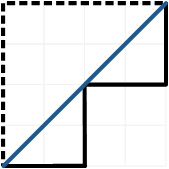
\includegraphics[width=\textwidth]{euclidean_manhattan_distance}
\end{column}
\begin{column}{.65\textwidth}
{\small \emph{Blue $\rightarrow$ Euclidean distance} \\
Black $\rightarrow$ Manhattan distance}
\end{column}
\end{columns}

\begin{exampleblock}{Question}
\begin{itemize}
\item What is the distance $d = \text{bottom left }\rightarrow\text{ top right}$ in $L^1$- and $L^2$-norm?
\begin{itemize}
\item $\norm{d}_1 = 8$, $\norm{d}_2 = 16$
\item $\norm{d}_1 = 8$, $\norm{d}_2 = \sqrt{32}$
\item $\norm{d}_1 = \sqrt{32}$, $\norm{d}_2 = 8$
\end{itemize}
\item \CourseQuiz
\end{itemize}
\end{exampleblock} 
%{\rightarrow $\norm{\text{bottom left }\rightarrow\text{ top right}}_1 = 8$, $\norm{\text{bottom left }\rightarrow\text{ top right}}_2 = \sqrt{4^2 + 4^2} = \sqrt{32}$
%}
\end{frame}

\begin{frame}[fragile]
  \frametitle{Vector Norms in R}
\begin{itemize}
\item No default built-in function, instead \emph{calculate the $L^1$- and $L^2$-norm manually}
<<>>=
x <- c(1, 2, 3)
sum(abs(x)) # L1-norm
sqrt(sum(x^2)) # L2-norm
@
\item The $p$-norm needs to be computed as follows
<<>>=
(sum(abs(x)^3))^(1/3) # 3-norm
@
\end{itemize}
\end{frame}

%\begin{frame}[fragile]
%  \frametitle{Matrix Norms}
%\begin{itemize}
%\item \emph{Matrix norms} are the natural extension of vector norms to matrices
%\item Definitions and numerical computations are often more difficult
%\item Common examples 
%\begin{itemize}
%\item The \emph{$p$-norm of a matrix $A$} is defined as 
%\begin{equation*} 
%\norm{A}_p = \max \left(\sum\limits_{i=1}^M{|a_{ij}|^p}\right)^{\frac{1}{p}} 
%\end{equation*}
%\item In R we can specify the one norm, infinity norm, frobenius norm and maximum modulus easily with the function \verb@norm()@
%\end{itemize}
%\begin{figure}
%\begin{minipage}{0.61\columnwidth}
%<<>>=
%m <- matrix(c(1,2,3,4,5,6),ncol=3)
%norm(m, type="O")
%norm(m, type="I")
%@
%\end{minipage}
%\begin{minipage}{0.38\columnwidth}
%<<>>=
%norm(m, type="F")
%norm(m, type="M")
%@
%\end{minipage}
%\end{figure}
%\end{frame}

\begin{frame}[fragile]
  \frametitle{Scalar Multiplication}
\begin{itemize}
\item Definition:
$
\lambda \vecval{x} =
\vecval{x} \lambda = 
\begin{bmatrix}
\lambda x_1 \\
\vdots \\
\lambda x_n
\end{bmatrix}
\qquad
\lambda A = 
A \lambda = 
\begin{bmatrix}
\lambda a_{11} & \cdots & \lambda a_{1m} \\
\vdots & \ddots & \vdots \\
\lambda a_{n1} & \cdots & a_{nm}
\end{bmatrix}
$
\item Use the \emph{default multiplication operator} \verb@*@
<<,size='scriptsize'>>=
5*c(1, 2, 3)
m <- matrix(c(1,2, 3,4, 5,6), ncol=3)
m
5*m
@
\end{itemize}
\end{frame}

\begin{frame}[fragile]
  \frametitle{Transpose}
\begin{itemize}
\item The \emph{transpose of a matrix} $A$ is another matrix $A^T$ where the \emph{values in columns and rows are flipped}
\begin{equation*}
A^T \define [a_{ji}]_{ij}
\end{equation*}
\item Example:
$\footnotesize
\begin{bmatrix}
1 & 3 & 5 \\
2 & 4 & 6
\end{bmatrix}^T = \begin{bmatrix}
1 & 2 \\
3 & 4 \\
5 & 6 \end{bmatrix}$
\item Transpose via \verb@t(A)@
<<,size='scriptsize'>>=
m
t(m)
@
\end{itemize}
\end{frame}

\begin{frame}[fragile]
  \frametitle{Matrix-by-Vector Multiplication}
\begin{itemize}
\item \emph{Definition:}
\begin{equation*}
\footnotesize
  A \vecval{x} =
  \left[
    \begin{array}{cccc}
      a_{11} & a_{12} & \ldots & a_{1m}\\
      a_{21} & a_{22} & \ldots & a_{2m}\\
      \vdots & \vdots & \ddots & \vdots\\
      a_{n1} & a_{n2} & \ldots & a_{nm}
    \end{array}
  \right]
  \left[
    \begin{array}{c}
      x_1\\
      x_2\\
      \vdots\\
      x_n
    \end{array}
  \right]
  =
  \left[
    \begin{array}{c}
      a_{11}x_1+a_{12}x_2 + \cdots + a_{1m} x_n\\
      a_{21}x_1+a_{22}x_2 + \cdots + a_{2m} x_n\\
      \vdots\\
      a_{n1}x_1+a_{n2}x_2 + \cdots + a_{nm} x_n\\
    \end{array}
  \right] 
\end{equation*}
with $A \in\R^{n \times m}$, $\vecval{x} \in\R^{n}$ and $A\vecval{x} \in\R^n$
\item Use \emph{operator \%*\%} in R
<<>>=
m %*% x
@
\end{itemize}
\end{frame}

\begin{frame}[fragile]
  \frametitle{Element-Wise Matrix Multiplication}
\begin{itemize}
\item For matrices $A \in\R^{n \times m}$ and $B \in\R^{n \times m}$, it returns a matrix $C \in\R^{n \times m}$ of defined as 
\begin{equation*}
c_{ij} = a_{ij} b_{ij}
\end{equation*}
\item The default multiplication operator \verb@*@ performs an \emph{element-wise multiplication}
<<>>=
m
m*m
@
\end{itemize}
\end{frame}

\begin{frame}[fragile]
  \frametitle{Matrix-by-Matrix Multiplication}
\begin{itemize}
\item Given matrices $A \in\R^{n \times m}$ and $B \in\R^{m \times l}$, then the \emph{matrix multiplication} obtains $C = AB \in\R^{n \times l}$, defined by
\begin{equation*}
c_{ij} = \sum_{k=1}^{m} a_{ik} b_{kj}
\end{equation*}
\item It is \emph{implemented by the operator} \%*\%
\end{itemize}
\vspace*{-0.4cm}
\begin{columns}[T]
\begin{column}{.45\textwidth}
<<,size='scriptsize'>>=
m
@
\end{column}
\begin{column}{.45\textwidth}
<<,size='scriptsize'>>=
t(m)
@
\end{column}
\end{columns}
<<,size='scriptsize'>>=
m %*% t(m)
@
\end{frame}

\begin{frame}[fragile]
  \frametitle{Identity Matrix}
\begin{itemize}
\item The \emph{identity matrix}
\begin{equation*}
I_n = \diag(1, 1, \ldots, 1) \in\R^{n \times n}
\end{equation*}
is a square matrix with $1$s on the diagonal and $0$s elsewhere
\item It fulfills 
\begin{equation*}
I_n A = A I_m = A
\end{equation*}
given a matrix $A \in\R^{n \times m}$
\item The command \verb@diag(n)@ creates an identity matrix of size $n \times n$
<<>>=
diag(3)
@
%\item In order to extract a matrix with only its \emph{diagonal elements} of the original matrix $A$, use \verb@diag(A)@
%<<>>=
%diag(A)
%@
%as defined by
\end{itemize}
\end{frame}

\begin{frame}[fragile]
  \frametitle{Matrix Inverse}
\begin{itemize}
\item The \emph{inverse} of a square matrix $A$ is a matrix $A^{-1}$ such that 
\begin{equation*}
A A^{-1} = I
\qquad
\text{(note that generally this is $\neq A^{-1} A$)}
\end{equation*}
\item A square matrix has an inverse \emph{if and only if its determinant $\det A \neq 0$}
\item The direct calculation is \emph{numerically highly unstable}, and thus one often rewrites the problem to \emph{solve a system of linear equations}
\end{itemize}
\end{frame}

\begin{frame}[fragile]
  \frametitle{Matrix Inverse in R}
\begin{itemize}
\item \verb@solve()@ calculates the inverse $A^{-1}$ of a square matrix $A$
<<message=FALSE,warning=FALSE>>=
sq.m <- matrix(c(1,2, 3,4), ncol=2)
sq.m
solve(sq.m)
sq.m %*% solve(sq.m) - diag(2) # post check
@
\end{itemize}
\end{frame}

\begin{frame}[fragile]
  \frametitle{Pseudoinverse}
\begin{itemize}
\item The \emph{pseudoinverse} $A^+ \in\R^{m \times n}$ is a \emph{generalization} of the inverse of a matrix $A \in\R^{n \times m}$; fulfilling among others
\begin{equation*}
A A^+ = I
\end{equation*}
\item \verb@ginv(A)@ inside the library \verb@MASS@ calculates the pseudoinverse 
<<MASS,eval=FALSE,size='scriptsize'>>=
library(MASS)
@
<<,include=FALSE,size='scriptsize'>>=
<<MASS>>
@
<<,size='scriptsize'>>=
ginv(m)
m %*% ginv(m) 
@
\item If $A A^+$ is invertible, it is given by 
\begin{equation*}
A^+ \define A^T \left(A A^T \right)^{-1}
\end{equation*}
\end{itemize}
\end{frame}

\begin{frame}[fragile]
  \frametitle{Determinant}
\begin{itemize}
\item The \emph{determinant} $\det A$ is a useful value for a square matrix $A$, relating to \eg the region it spans
\item A square matrix is also invertible if and only if $\det A \neq 0$
\end{itemize}
\textbf{Calculation}
\begin{itemize}
\item The determinant of of a $2 \times 2$ matrix $A$ is defined by
\begin{equation*} 
\det A = \begin{vmatrix} a_{11} & a_{12} \\
a_{21} & a_{22} \end{vmatrix} = a_{11} a_{22} - a_{12} a_{21}
\end{equation*}
\item A similar simple rule exists for matrices of size $3 \times 3$, for all others one usually utilizes the \emph{Leibniz or the Laplace formula}
\item Calculation in R is via \verb@det(A)@
\end{itemize}
<<>>=
det(sq.m)
@
\end{frame}

\begin{frame}[fragile]
  \frametitle{Eigenvalues and Eigenvectors}
\begin{itemize}
\item An \emph{eigenvector} $\vecval{v}$ of a square matrix $A$ is a \emph{vector that does not change its direction under the linear transformation} by $A \in \R^{n \times n}$
\item This is given by \begin{equation*}
A \vecval{v} = \lambda \vecval{v} \qquad \text{for } \vecval{v} \neq \left[ 0, \ldots 0 \right]^T \in\R^{n}
\end{equation*}
where $\lambda \in\R$ is the \emph{eigenvalue} associated with the eigenvector $\vecval{v}$
\item Example: the matrix 
$A = \begin{bmatrix}
2 & 0 & 1 \\
0 & 2 & 0 \\
1 & 0 & 2
\end{bmatrix}$
has the following eigenvectors and eigenvalues
\begin{equation*}
\lambda_1 = 1, \vecval{v}_1 = \begin{bmatrix} 1 \\ 0 \\ -1 \end{bmatrix},
\quad
\lambda_2 = 2, \vecval{v}_2 = \begin{bmatrix} 0 \\ 1 \\ 0 \end{bmatrix},
\quad
\lambda_3 = 3, \vecval{v}_3 = \begin{bmatrix} 1 \\ 0 \\ 1 \end{bmatrix}
\end{equation*}
\end{itemize}
\end{frame}

\begin{frame}[fragile]
  \frametitle{Eigenvalues and Eigenvectors}
\textbf{Geometric interpretation}

\begin{columns}[T]
\begin{column}{.5\textwidth}
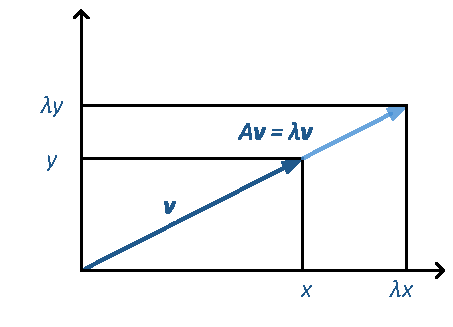
\includegraphics[width=\textwidth]{eigenvalue_equation}
\end{column}
\begin{column}{.4\textwidth}
{\small Matrix $A$ \emph{stretches} the vector $\vecval{v}$ but does \emph{not change its direction}\\
$\rightarrow$ $\vecval{v}$ is an eigenvector of $A$}
\end{column}
\end{columns}
\end{frame}

\begin{frame}[fragile]
  \frametitle{Eigenvalues and Eigenvectors}
\begin{exampleblock}{Question}
\begin{itemize}
\item Given $A = \begin{bmatrix}
1 & 0 & 0 \\
1 & 2 & 0 \\
2 & 3 & 3
\end{bmatrix}$
\item Which of the following is not an eigenvector/eigenvalue pair?
\begin{itemize}
\item $\lambda_1 = 1$, $\vecval{v}_1 = \begin{bmatrix} \frac{2}{3} \\ -\frac{2}{3} \\ \frac{1}{3} \end{bmatrix}$
\item $\lambda_2 = 2$, $\vecval{v}_2 = \begin{bmatrix} 2 \\ 1 \\ 1 \end{bmatrix}$
\item $\lambda_3 = 3$, $\vecval{v}_3 = \begin{bmatrix} 0 \\ 0 \\ 1 \end{bmatrix}$
\end{itemize}
\item \CourseQuiz
\end{itemize}
\end{exampleblock}
%{$\rightarrow$ $\lambda_2$, $\vecval{v}_2$
%}
\end{frame}

\begin{frame}[fragile]
  \frametitle{Eigenvalues and Eigenvectors in R}
\begin{itemize}
\item Eigenvalues and eigenvectors of a square matrix $A$ via \verb@eigen(A)@
<<>>=
sq.m
e <- eigen(sq.m)
e$val # eigenvalues
e$vec # eigenvectors
@
\end{itemize}
\end{frame}

\begin{frame}[fragile]
  \frametitle{Definiteness of Matrices}
\begin{itemize}
\item The \emph{definiteness} of a matrix helps in determining the \emph{nature of optima}
\item Definitions
\begin{itemize}
\item The \emph{symmetric} matrix $A \in\R^{n \times n}$ is \emph{positive definite} if
\begin{equation*}
\vecval{x}^T A \vecval{x} > 0 \quad\text{for all } \vecval{x} \neq \left[0, \ldots, 0\right]^T
\end{equation*}
\item The \emph{symmetric} matrix $A \in\R^{n \times n}$ is \emph{positive semi-definite} if
\begin{equation*}
\vecval{x}^T A \vecval{x} \geq 0 \quad\text{for all } \vecval{x} \neq \left[0, \ldots, 0\right]^T
\end{equation*} 
\end{itemize}
\end{itemize}
\textbf{Example}\\
The identity matrix 
$I_2 = \begin{bmatrix}
1 & 0 \\
0 & 1 
\end{bmatrix}$
is positive definite, since
\begin{equation*}
\vecval{x}^T I_2 \vecval{x} = \left[ x_1, x_2 \right]
\begin{bmatrix}
1 & 0 \\
0 & 1
\end{bmatrix}
\begin{bmatrix}
x_1 \\
x_2
\end{bmatrix}
= x_1^2 + x_2^2 > 0 \text{ for all } \vecval{x} \neq \left[ 0, 0 \right]^T
\end{equation*}
\end{frame}

\begin{frame}[fragile]
  \frametitle{Positive Definiteness}
\begin{itemize}
\item \emph{Tests} for positive definiteness
\begin{itemize}
\item Evaluating $\vecval{x}^T A \vecval{x}$ for all $\vecval{x}$ is impractical
\item All eigenvalues $\lambda_i$ of $A$ are positive
\item Check if all upper-left sub-matrices have positive determinants (Sylvester's criterion)
\end{itemize}
\end{itemize}
% TODO: example for Sylvester's criterion
\end{frame}

\begin{frame}[fragile]
  \frametitle{Definiteness Tests in R}
The library \verb@matrixcalc@ offers methods to test all variants of definiteness
<<matrixcalc,eval=FALSE>>=
library(matrixcalc)
@
<<,include=FALSE>>=
<<matrixcalc>>
@
\vspace*{-0.4cm}
\begin{columns}[T]
\begin{column}{.35\textwidth}
%is.indefinite(I)
<<,size='scriptsize'>>=
I <- diag(3)
I
is.negative.definite(I)
is.positive.definite(I)
@
\end{column}
\begin{column}{.55\textwidth}
<<,size='scriptsize', tidy=FALSE>>=
C <- matrix(c(-2,1,0, 1,-2,1, 0,1,-2), 
            nrow=3, byrow=TRUE)
C
is.positive.semi.definite(C)
is.negative.semi.definite(C)
@
\end{column}
\end{columns}
\end{frame}

\section{Differentiation}

%\begin{frame}
  %\frametitle{Continuity}
%\textbf{Definition}\\
%Let $f : D \subseteq \R^n \rightarrow \R$ be a function and $x_0 \in D$
%\begin{enumerate}
%\item $f$ is \emph{continuous at $x_0$} if $\lim_{x\to x_0} f(x) = f(x_0)$
%\item $f$ is continuous on $D$ if it is continuous at each point of $D$
%\end{enumerate}
%\end{frame}

\begin{frame}
  \frametitle{Differentiability}
\textbf{Definition}\\
Let $f : D \subseteq \R^n \rightarrow \R$ be a function and $x_0 \in D$
\begin{itemize}
\item $f$ is \emph{differentiable at the point $x_0$} if the following limit exists
\begin{equation*}
f'(x_0) = \frac{\dd f}{\dd x}(x_0) = \lim_{\varepsilon \to 0}\frac{f(x_0 + \varepsilon) - f(x_0)}{\varepsilon}
\end{equation*}
the limit $f'(x_0)$ is called the \emph{derivative of $f$ at the point $x_0$}
\item If it is differentiable for all $x \in D$, then $f$ is \emph{differentiable} with \emph{derivative $f'$}
\end{itemize}

\vspace*{0.4cm}
\textbf{Remarks}
\begin{itemize}
\item Similarly, the 2nd derivative $f''$ and, by induction, the \emph{$n$-th derivative $f^{(n)}$}
\item Geometrically, $f'(x_0)$ is the \emph{slope of the tangent} to $f(x)$ at $x_0$
\end{itemize}
\end{frame}

\begin{frame}
  \frametitle{Differentiability}
\textbf{Examples}\\
\begin{tabular}{ccc}
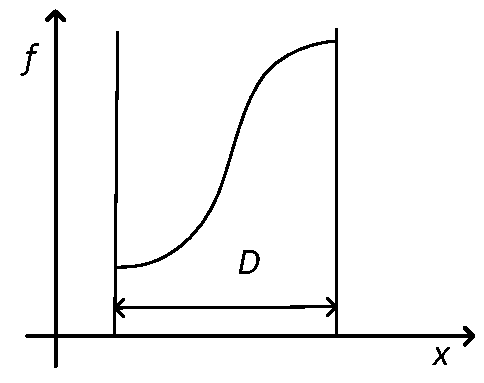
\includegraphics[width=.3\textwidth]{continuous} & 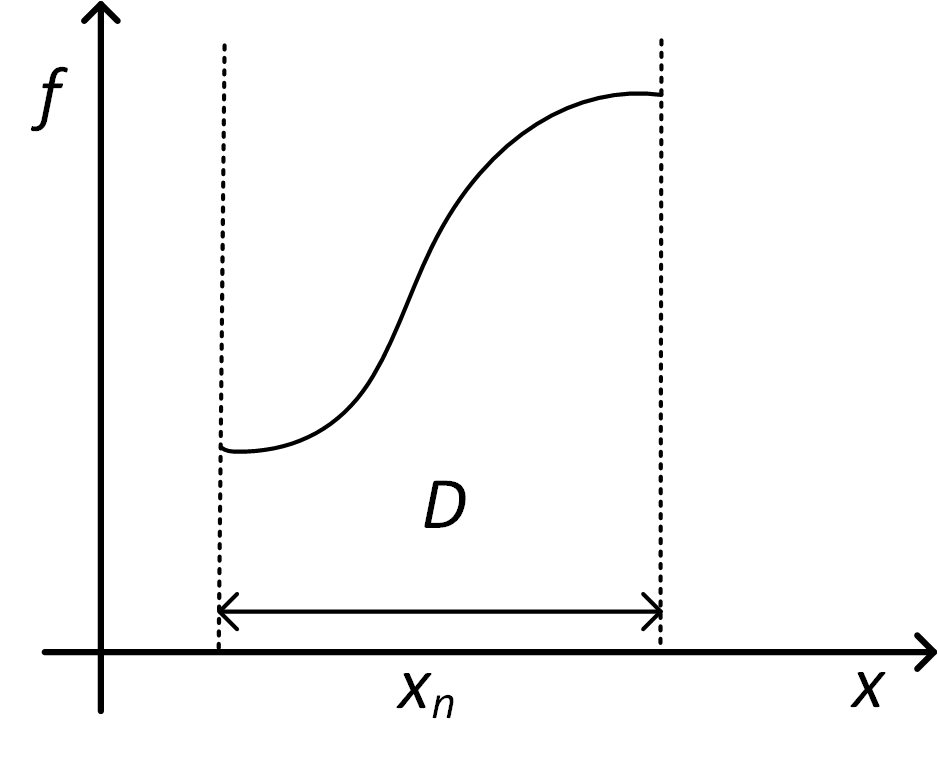
\includegraphics[width=.3\textwidth]{non-differentiable_continuous} & 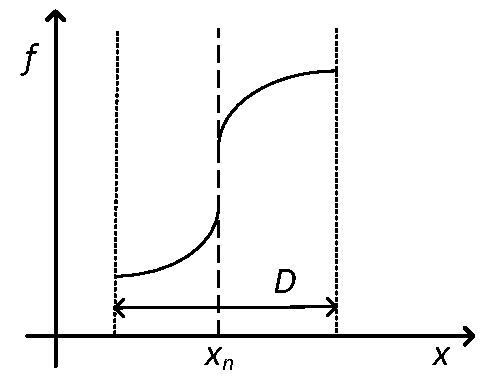
\includegraphics[width=.3\textwidth]{non-differentiable_discontinuous} \\
continuous & continuous & discontinuous \\
differentiable & not differentiable & not differentiable
\end{tabular}

\begin{exampleblock}{Question}
\begin{itemize}
\item What is correct for the function $f(x) = \frac{2x-1}{x+2}$?
\begin{itemize}
\item Continuous and differentiable
\item Continuous but not differentiable
\item Discontinuous and not differentiable
\end{itemize}
\item \CourseQuiz
\end{itemize}
\end{exampleblock}
%{$\rightarrow$ Discontinuous and not differentiable
%}
\end{frame}

\begin{frame}
  \frametitle{Chain Rule}
Let $v(x)$ be a differentiable function, then the \emph{chain rule} gives
\begin{equation*}
\frac{\dd u(v(x))}{\dd x} = \frac{\dd u}{\dd v} \frac{\dd v}{\dd x} 
\end{equation*}

\vspace*{0.3cm}
\textbf{Example} Given 
%\begin{equation*}
$u(v(x)) = \sin{(\pi x)}$, 
%\end{equation*}
 then $u = \sin$, $v(x) = \pi x$ and
\begin{equation*}
\frac{\dd u(v(x))}{\dd x} = \frac{\dd \sin{(\pi x)}}{\dd v} \frac{\dd (\pi x)}{\dd x} = \cos{(\pi x)} \pi 
\end{equation*}

\begin{exampleblock}{Question}
\begin{itemize}
\item What is the derivative of $\log{4-x}$?
\begin{itemize}
\item $\frac{1}{x-4}$
\item $\frac{4}{x}$
\item $\frac{1}{4-x}$
\end{itemize}
\item \CourseQuiz
\end{itemize}
\end{exampleblock}
%{$\rightarrow$ $= \cfrac{1}{4-x} \cfrac{\dd}{\dd x}(4-x) = \cfrac{1}{4-x} (-1) = \cfrac{1}{x-4}$
%
\end{frame}

\begin{frame}
  \frametitle{Partial Derivative}
\begin{itemize}
\item The \emph{partial derivative} with respect to $x_i$ is given by 
\begin{equation*}
\frac{\partial f}{\partial x_i}(\vecval{x}) \define \lim_{\varepsilon \to 0} \frac{f(x_1, \ldots, x_i + \varepsilon, \ldots, x_n) - f(x_1, \ldots, x_i, \ldots, x_n)}{\varepsilon}
\end{equation*}
\item $f$ is called \emph{partially differentiable}, if $f$ is differentiable at \emph{each} point with respect to \emph{all} variables
\item Partial derivatives can be \emph{exchanged in their order}
\begin{equation*}
\frac{\partial}{\partial x_i} \left( \frac{\partial f}{\partial x_j} \right) = \frac{\partial}{\partial x_j} \left( \frac{\partial f}{\partial x_i} \right)
\end{equation*}
\end{itemize}
\end{frame}

%\begin{frame}
  %\frametitle{Derivatives}
%\begin{itemize}
%\emph{Derivative} measures the sensitivity of a function to its input values
%\begin{equation*}
%f'(x) = \frac{\d f}{\d x} f 
%\qquad
%f'(x, y) = \frac{\partial f}{\partial x}(x, y)
%\end{equation*}
%\item Gradient of $f : \R^n \rightarrow \R^n$
%\begin{equation*}
%\nabla f(\vecval{x}) = \left( \frac{\partial f}{\partial x_1}(a), \ldots, \frac{\partial f}{\partial x_n}(a) \right)
%\end{equation*}
%given differentiability
%\end{itemize}
%%\textbf{Rules}
%%\begin{itemize}
%%\item Power rule: $f(x) = x^r$, then $f'(x) = r x^{r-1}$
%%\item Sum rule: $(\alpha f + \beta g)' = \alpha f' + \beta g'$
%%\item Product rule: $(fg)' = f'g + fg'$
%%\item Chain rule: $f(x) = h(g(x))$, then $f'(x) = h'(g(x)) \cdot g'(x)$
%%\end{itemize}
%\end{frame}

\begin{frame}[fragile]
  \frametitle{Derivatives in R}
\begin{itemize}
\item The function \verb@D(f, "x")@ \emph{derives an expression $f$ symbolically}
<<>>=
f <- expression(x^5 + 2*y^3 + sin(x) - exp(y))

D(f, "x")
D(D(f, "y"),"y")
D(D(f, "x"),"y")
@
\item To \emph{compute the derivative at a specific point}, we use \verb@eval(expr)@
<<>>=
eval(D(f, "x"), list(x=2, y=1))
@
\end{itemize}
\end{frame}

\begin{frame}
  \frametitle{Finite Differences}
\begin{itemize}
\item Numerical methods to \emph{approximate derivatives numerically}
\item Use a \emph{step size} $h$, usually of order $10^{-6}$
\end{itemize}
\begin{columns}[T]
\begin{column}{.5\textwidth}
\begin{itemize}
\item \emph{Forward} differences
\begin{equation*}
f'(x) = \frac{f(x + h) - f(x)}{h}
\end{equation*}
\item \emph{Backward} differences
\begin{equation*}
f'(x) = \frac{f(x) - f(x - h)}{h}
\end{equation*}
\item \emph{Centered} differences
\begin{equation*}
f'(x) = \frac{f(x + h) - f(x - h)}{2h}
\end{equation*}
\end{itemize}
\end{column}
\begin{column}{.4\textwidth}
\hspace*{-0.5cm}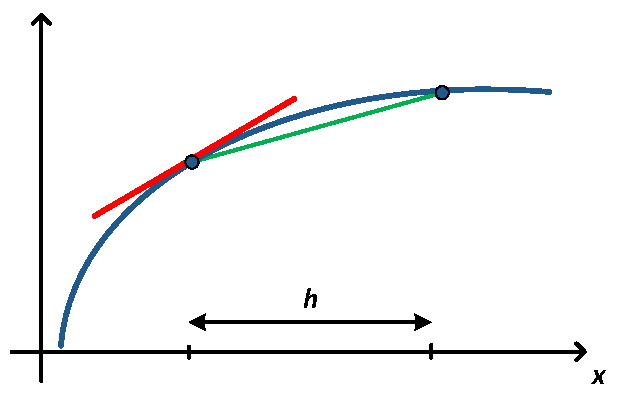
\includegraphics[width=1.2\textwidth]{finite_difference_approximation}
\end{column}
\end{columns}
\end{frame}

\begin{frame}
  \frametitle{Higher-Order Differences}
Use the previous formulae to derive \emph{2nd order central differences}
\begin{align*}
f''(x) \approx & \frac{f'(x+h) - f'(x)}{h} \\
\approx & \frac{\cfrac{f(x+h)-f(x)}{h} - \cfrac{f(x)-f(x-h)}{h}}{h} \\
= & \frac{f(x+h) - 2f(x) + f(x-h)}{h^2}
\end{align*}
\end{frame}

\begin{frame}[fragile]
  \frametitle{Finite Differences in R}
\begin{exampleblock}{Question}
\begin{itemize}
\item Given $f(x) = \sin{x}$
\item Set \verb@h <- 10e-6@
\item How to calculate the derivative at $x = 2$ with centered differences in R?
\begin{itemize}
\item \verb@(sin(2+h) - sin(2-h)) / (2*h)@
\item \verb@(sin(2+h) - sin(2-h)) / 2*h@
\item \verb@(sin(2+h) - sin(2)) / (2*h)@
\end{itemize}
\item \CourseQuiz
\end{itemize}
\end{exampleblock}
%{$\rightarrow$ \verb@(sin(2+h) - sin(2-h)) / (2*h)@
%
\end{frame}

\begin{frame}
  \frametitle{Gradient and Hessian Matrix}
\begin{itemize}
\item \emph{Gradient} of $f : \R^n \rightarrow \R^n$
\begin{equation*}
\nabla f(\vecval{x}) = 
\begin{bmatrix} \cfrac{\partial f}{\partial x_1}(\vecval{x}) \\
\vdots \\
\cfrac{\partial f}{\partial x_n}(\vecval{x})
\end{bmatrix}
\end{equation*}
\item The second derivatives of $f$ are called the \emph{Hessian (matrix)}
\begin{equation*}
H(\vecval{x}) = \nabla^2 f(\vecval{x}) = 
\begin{bmatrix}
\frac{\partial^2 f}{\partial x_1^2}(\vecval{x}) & \cdots & \frac{\partial^2 f}{\partial x_1 \partial x_n}(\vecval{x}) \\
\vdots & \ddots & \vdots \\
\frac{\partial^2 f}{\partial x_n \partial x_1}(\vecval{x}) & \cdots & \frac{\partial^2 f}{\partial x_n^2}(\vecval{x})
\end{bmatrix}
\end{equation*}
\item Since the order of derivatives can be exchanged, the Hessian $H(\vecval{x})$ is \emph{symmetric}, \ie
%\begin{equation*}
$H(\vecval{x}) = \left( H(\vecval{x}) \right)^T$
%\end{equation*}
\end{itemize}
\end{frame}

\begin{frame}[fragile]
  \frametitle{Hessian Matrix in R}
\begin{itemize}
\item \verb@optimHess(x, f, ...)@ \emph{approximates the Hessian matrix} of $f$
<<>>=
f <- function(x) (x[1]^3*x[2]^2 - x[2]^2 + x[1])
optimHess(c(3, 2), f, control=(ndeps=0.0001))
@
\item Above example: forward differences to approximate the Hessian Matrix of $f(x_1, x_2)$ at a given point $(x_1, x_2)=(3,2)$ with a given step size $h=0.0001$
\end{itemize}
\end{frame}

\section{Taylor Approximation}

\begin{frame}[fragile]
  \frametitle{Taylor Series}
\begin{itemize}
\item Simple \emph{polynomial approximation} to almost arbitrary functions
\item \emph{Taylor series approximates} $f$ around a point $x_0$ as a \emph{power series}
\begin{align*} 
f(x) &= f(x_0)+\frac{f'(x_0)}{1!}(x-x_0)+\frac{f''(x_0)}{2!}(x-x_0)^2\\
& \qquad\qquad\qquad
+\frac{f'''(x_0)}{3!}(x-x_0)^3+\ldots \\
&= \sum\limits_{n=0}^\infty{\frac{f^{(n)}(x_0)}{n!}(x-x_0)^n}.
\end{align*}
\item $f$ must be \emph{infinitely differentiable}
\item If $x_0=0$ the series is also called \emph{Maclaurin series}
\item To \emph{obtain an approximation} of $f$, cut off after order $n$
\end{itemize}
\end{frame}

\begin{frame}[fragile]
  \frametitle{Taylor Approximation}
Approximation of order $n$ (\textcolor{CustomBlue}{blue}) around $x_0 = 0$ for $f(x) = \sin{x}$ (in \textcolor{darkgray}{gray})
<<taylor_sin,fig.show='animate',echo=FALSE,eval=TRUE,crop=TRUE,message=FALSE,warning=FALSE,fig.width=6,fig.height=4,out.width='.8\\linewidth'>>=
library(pracma)

f <- function(x) sin(x)
x0 <- 0
x <- seq(-10, 10, by=0.01)
y.f <- f(x)

for (o in seq(1, 11, by=1)) {
  taylor.poly <- taylor(f, x0=x0, n=o)
  y.taylor <- polyval(taylor.poly, x)
  plot(x, y.f, type = "l", col = "gray", lwd = 3, ylim=c(-10, +10), main=paste("n=", o, sep=""), ylab="f(x)")
  lines(x, y.taylor, col = "darkblue")
	points(x0, f(x0), pch=16, col="black")
  #grid()
}
@
\end{frame}

\begin{frame}[fragile]
  \frametitle{Taylor Approximation}
Approximation of order $n$ (\textcolor{CustomBlue}{blue}) around $x_0 = 0$ for $f(x) = \mathsf{e}^x$ (in \textcolor{darkgray}{gray})
<<taylor_e,fig.show='animate',echo=FALSE,eval=TRUE,crop=TRUE,message=FALSE,warning=FALSE,fig.width=6,fig.height=4,out.width='.8\\linewidth'>>=
library(pracma)

f <- function(x) exp(x)
x0 <- 0
x <- seq(-2.5, 2.5, by=0.01)
y.f <- f(x)

for (o in 1:8) {
  taylor.poly <- taylor(f, x0=x0, n=o)
  y.taylor <- polyval(taylor.poly, x)
  plot(x, y.f, type = "l", col = "gray", lwd = 3, ylim=c(-5, +20), main=paste("n=", o, sep=""), ylab="f(x)")
  lines(x, y.taylor, col = "darkblue")
	points(x0, f(x0), pch=16, col="black")
  #grid()
}
@
\end{frame}

\begin{frame}[fragile]
  \frametitle{Taylor Approximation}
Approximation of order $n$ (\textcolor{CustomBlue}{blue}) around $x_0 = 0$ for $f(x) = \log{x+1}$ (in \textcolor{darkgray}{gray})
<<taylor_log,fig.show='animate',echo=FALSE,eval=TRUE,crop=TRUE,message=FALSE,warning=FALSE,fig.width=6,fig.height=4,out.width='.8\\linewidth'>>=
library(pracma)

f <- function(x) log(x+1)
x0 <- 0
x <- seq(-1.5, 1.5, by=0.01)
y.f <- f(x)

for (o in seq(1, 11, by=2)) {
  taylor.poly <- taylor(f, x0=x0, n=o)
  y.taylor <- polyval(taylor.poly, x)
  plot(x, y.f, type = "l", col = "gray", lwd = 3, ylim=c(-4, +2), main=paste("n=", o, sep=""), ylab="f(x)")
  lines(x, y.taylor, col = "darkblue")
	points(x0, f(x0), pch=16, col="black")
  #grid()
}
@
\end{frame}

\begin{frame}[fragile]
  \frametitle{Taylor Series}
\begin{exampleblock}{Question}
\begin{itemize}
\item What is the Taylor series for $f(x) = \cfrac{1}{1-x}$ with $x_0 = 0$?
\begin{itemize}
\item $f(x) = \frac{1}{x} + 1 + x + x^2 + x^3 + \ldots$
\item $f(x) = 1 + x + x^2 + x^3 + \ldots$
\item $f(x) = x + x^2 + x^3 + \ldots$
\end{itemize}
\item \CourseQuiz
\end{itemize}
\end{exampleblock}
%{$\rightarrow$ $f(x) = 1 + x + x^2 + x^3 + \ldots$
%}
\pause
\begin{exampleblock}{Question}
\begin{itemize}
\item What is the Taylor series for $f(x) = \mathsf{e}^{x}$ with $x_0 = 0$?
\begin{itemize}
\item $f(x) = \frac{x}{1!} + \frac{x^2}{2!} + \frac{x^3}{3!} + \ldots$
\item $f(x) = 1 + \frac{x}{1} + \frac{x^2}{2} + \frac{x^3}{3} + \ldots$
\item $f(x) = 1 + \frac{x}{1!} + \frac{x^2}{2!} + \frac{x^3}{3!} + \ldots$
\end{itemize}
\item \CourseQuiz
\end{itemize}
\end{exampleblock}
%{$\rightarrow$ $f(x) =  1 + \frac{x}{1!} + \frac{x^2}{2!} + \frac{x^3}{3!} + \ldots$
%}
\end{frame}

%\begin{frame}[fragile]
  %\frametitle{Taylor Series}
%\textbf{Examples}
%\begin{itemize}
%\item \emph{$f(x) = \cfrac{1}{1-x}$} with $x_0 = 0$
%\begin{equation*} 
%f(x) = 1 + x + x^2 + x^3 + \ldots
%\end{equation*} 
%\item \emph{$f(x) = \cfrac{1}{x}$} with $x_0 = 1$
%\begin{equation*} 
%f(x) = 1 - (x-1) + (x-1)^2 - (x-1)^3 + \ldots
%\end{equation*} 
%\item \emph{$f(x) = \log{x}$} with arbitrary $x_0$
%\begin{equation*} 
%f(x) = \log{x_0} + \frac{1}{x_0}(x-x_0) - \frac{1}{x_0^2}\frac{(x-x_0)^2}{2} + \ldots
%\end{equation*} 
%\item \emph{$f(x) = \mathsf{e}^{x}$} with $x_0 = 0$
%\begin{equation*} 
%f(x) = 1 + \frac{x}{1!} + \frac{x^2}{2!} + \frac{x^3}{3!} + \ldots
%\end{equation*}
%\end{itemize}
%\end{frame}

\begin{frame}[fragile]
  \frametitle{Taylor Approximation with R}
\begin{itemize}
\item Load library \verb@pracma@
<<pracma,eval=FALSE,size='scriptsize'>>=
library(pracma)
@
<<,include=FALSE,size='scriptsize'>>=
<<pracma>>
@
\item \emph{Calculate approximation} up to degree $4$ with \verb@taylor(f, x0, n)@
<<,size='scriptsize'>>=
f <- function(x) cos(x)
taylor.poly <- taylor(f, x0=0, n=4)
taylor.poly
@
\item \emph{Evaluate Taylor approximation} \verb@p@ at $x$ with \verb@polyval(p, x)@
<<,size='scriptsize'>>=
polyval(taylor.poly, 0.1) # x = 0.1
cos(0.1) # for comparison
polyval(taylor.poly, 0.5) - cos(0.5)
@
\end{itemize}
\end{frame}

\begin{frame}[fragile]
  \frametitle{Taylor Approximation in R}
Visualizing Taylor approximation

<<plot_taylor,fig.width=6,fig.height=4,out.width='.7\\linewidth',size='scriptsize',tidy=FALSE,fig.keep='last'>>=
x <- seq(-7.0, 7.0, by=0.01)
y.f <- f(x)
y.taylor <- polyval(taylor.poly, x)
plot(x, y.f, type="l", col="gray", lwd=2, ylim=c(-1, +1))
lines(x, y.taylor, col="darkblue")
grid()
@
\end{frame}

\section{Optimality Conditions}

\begin{frame}
  \frametitle{Extreme Value Theorem}
\textbf{Theorem}
\begin{itemize}
\item Given: real-valued function $f$
\item $f$ continuous in the closed and bounded interval $[x_{L}, x_{U}]$
\item Then $f$ must \emph{attain a maximum and minimum at least once}
\item I.\,e. there exists $x_{\max}, x_{\min} \in [x_{L}, x_{U}]$ such that
\begin{equation*}
f(x_{\max}) \geq f(x) \geq f(x_{\min}) \qquad\text{for all } x \in [x_{L}, x_{U}]
\end{equation*}
\end{itemize}

\hspace*{1cm}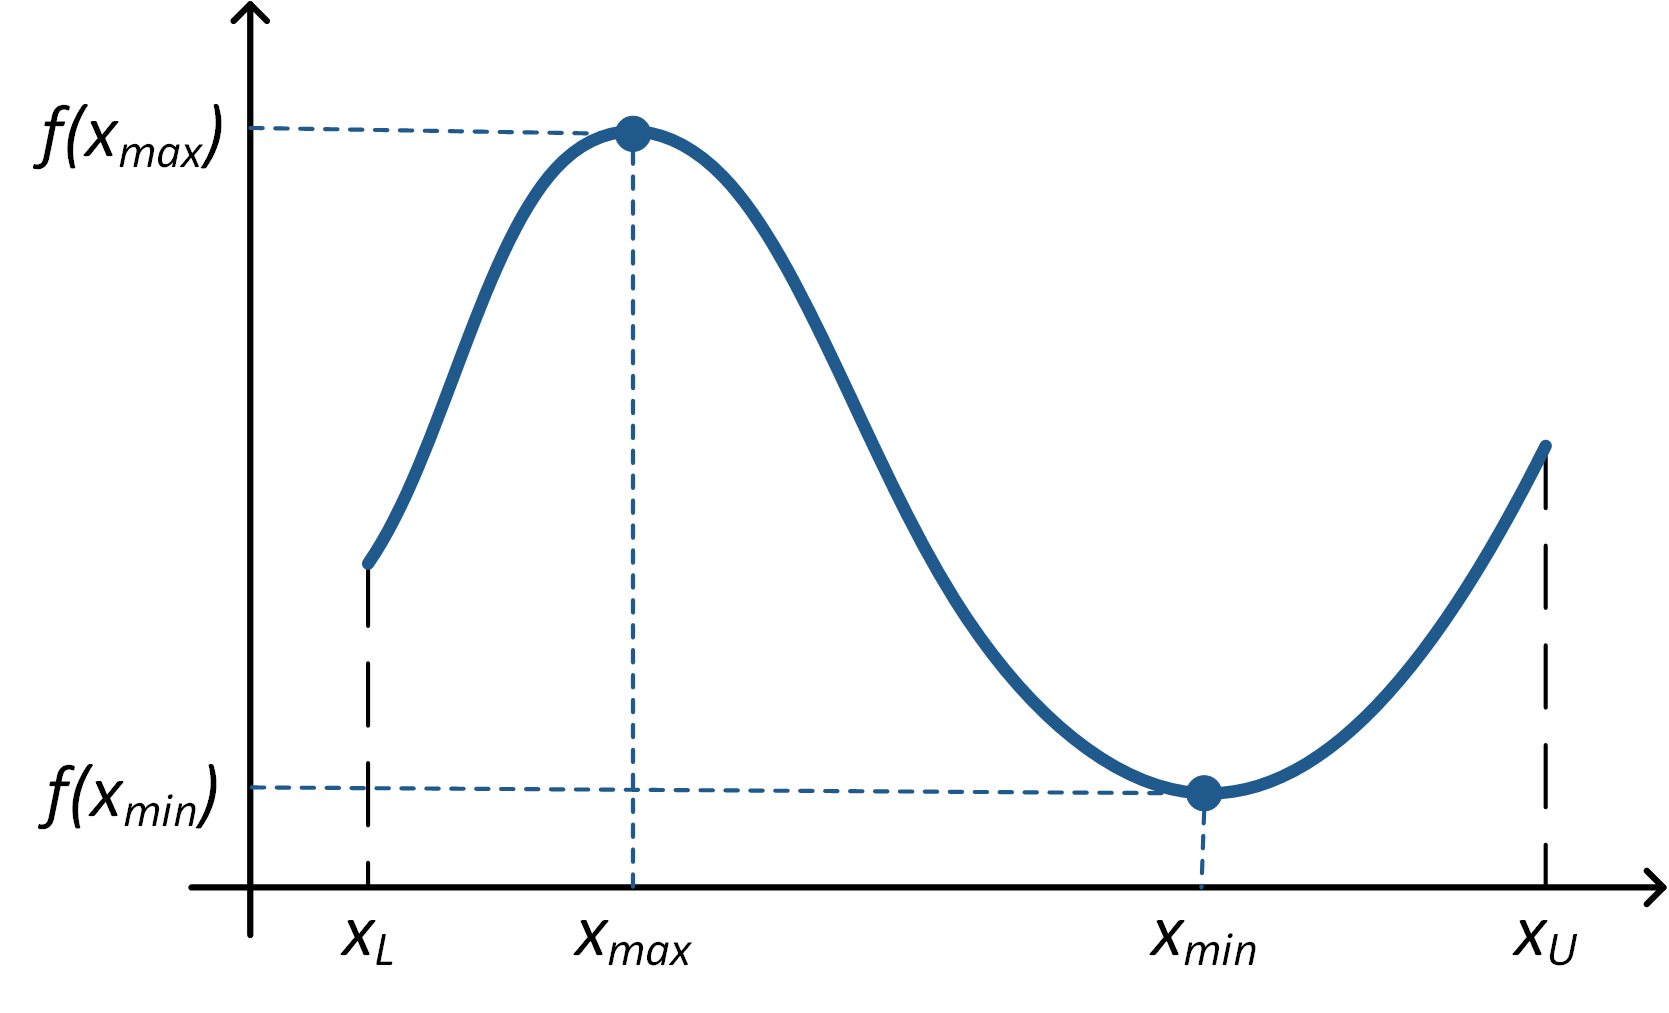
\includegraphics[width=.55\textwidth]{extreme_value_theorem}
\end{frame}

\begin{frame}
  \frametitle{Optimum}
\textbf{Definitions}
\begin{columns}[T]
\begin{column}{\textwidth}
\begin{itemize}
\item $x^\ast$ is a \emph{local minimum} if $x^\ast \in D$ and if there is a neighborhood $N(x^\ast)$, such that
\begin{equation*}
f(x^\ast) \leq f(x) \qquad \text{for all } x \in N(x^\ast) \subseteq D
\end{equation*}
\item $x^\ast$ is a \emph{strict local minimum} if $x^\ast \in D$ and if there is a neighborhood $N(x^\ast)$, such that
\begin{equation*}
f(x^\ast) < f(x) \qquad \text{for all } x \in N(x^\ast) \subseteq D
\end{equation*}
\end{itemize}
\end{column}
\end{columns}

\begin{columns}[T]
\begin{column}{.75\textwidth}
\begin{itemize}
\item $x^\ast$ is a \emph{global minimum} if $x^\ast \in D$ and
\begin{equation*}
f(x^\ast) \leq f(x) \qquad \text{for all } x \in D
\end{equation*}
\end{itemize}

$\rightarrow$ What conditions need to be fulfilled for a minimum?
\end{column}
\begin{column}{.25\textwidth}
\hspace*{-0.5cm}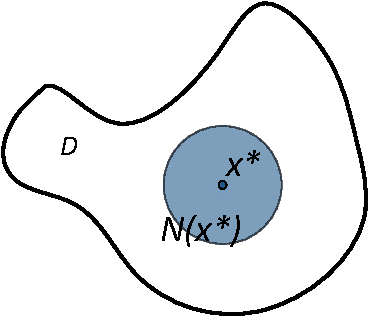
\includegraphics[width=1.2\textwidth]{neighborhood}
\end{column}
\end{columns}
\end{frame}

\begin{frame}
  \frametitle{Optimality Condition}
\emph{Conditions} for a minimum $x^\ast$

\vspace*{0.2cm}
\begin{center}
\begin{tabular}{lll}
1st order condition & $f'(x^\ast) = 0$ & \textit{$\rightarrow$ necessary} \\
2nd order condition & $f''(x^\ast) > 0$ & \textit{$\rightarrow$ sufficient}
\end{tabular}
\end{center}

\vspace*{0.4cm}
\begin{columns}[T]
\begin{column}{.65\textwidth}
\emph{Interpretation} through Taylor series\\
\qquad $f(x + h) = f(x) + f'(x) h + \Oh{h^2}$\\
Then
\begin{equation*}
\footnotesize
\left.
\begin{split}
f(x+h) - f(x) & \geq 0 \\
f(x-h) - f(x) & \geq 0
\end{split}
\right\}
\Rightarrow f'(x) = 0
\end{equation*}
%and
\begin{equation*}
\footnotesize
\left.
\begin{split}
f(x+h) - f(x) & = \frac{1}{2} f''(x) h^2 + \Oh{h^3} & > 0 \\
f(x-h) - f(x) & = \frac{1}{2} f''(x) h^2 + \Oh{h^3} & > 0
\end{split}
\right\}
\Rightarrow f''(x) > 0
\end{equation*}
\end{column}
\begin{column}{.3\textwidth}
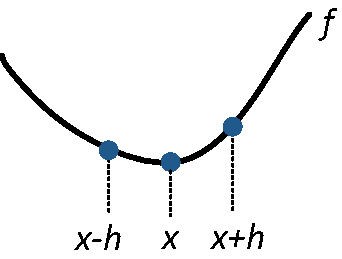
\includegraphics[width=\textwidth]{function_steps_h}
\end{column}
\end{columns}
\end{frame}

\begin{frame}
  \frametitle{Optimality Condition}
\textbf{Theorem} (\emph{sufficient} optimality condition)\\
Let $f$ be twice continuously differentiable and let $\vecval{x}^\ast \in \R^n$, if
\begin{enumerate}
\item First order condition
\begin{equation*}
\nabla f(\vecval{x}^\ast) = \left[ 0, \ldots, 0 \right]^T
\end{equation*}
\item Second order condition
\begin{equation*}
\nabla^2 f(\vecval{x}^\ast) \text{ is positive definite}
\end{equation*}
\end{enumerate}
then $\vecval{x}^\ast$ is a \emph{strict local minimizer}
\vspace*{0.4cm}
\end{frame}

\begin{frame}
  \frametitle{Optimality Conditions}
The previous theory does not cover all cases
\begin{itemize}
\item Imagine $f(x) = \abs{x}$
\end{itemize}
\vspace*{-1cm}
\begin{center}
<<abs,fig.width=4,fig.height=3,out.width='.7\\linewidth',echo=FALSE,eval=TRUE,keep='last'>>=
x <- seq(-3.0, 3.0, by=0.01)
y.f <- abs(x)
plot(x, y.f, type="l", col="darkblue", lwd=2, ylab="abs(x)")
grid()
@
\end{center}
\vspace*{-1cm}
\begin{itemize}
\item $f(x)$ has a global minimum at $x^\ast = 0$
\item Since $f$ is \emph{not differentiable}, the \emph{optimality conditions do not apply}
\end{itemize}
\end{frame}

\begin{frame}
  \frametitle{Stationarity}
\textbf{Definition}
\begin{itemize}
\item Let $f$ be continuously differentiable. A point $\vecval{x}^\ast \in\R^{n}$ is \emph{stationary} if
\begin{equation*}
\nabla f(\vecval{x}^\ast) = 0
\end{equation*}
\item $\vecval{x}^\ast$ is called a \emph{saddle point} if it is neither a local minimum or maximum
\end{itemize}

\vspace*{0.4cm}
\textbf{Examples}
\begin{columns}[T]
\begin{column}{.6\textwidth}
\begin{itemize}
\item $f(x) = -x^2$ has only one stationary $x^\ast = 0$, since $\nabla f(x^\ast) = -2 x^\ast = 0$
\item $f(x) = x^3$ has a saddle point at $x^\ast = 0$
\item $f(x_1, x_2) = x_1^2 - x_2^2$ has a saddle point $\vecval{x}^\ast = \left[ 0, 0 \right]^T$
\end{itemize}
\end{column}
\begin{column}{.35\textwidth}
\vspace*{-2cm}
\hspace*{-5cm}%
<<saddle_point,fig.width=6,fig.height=4,out.width='3.\\textwidth',echo=FALSE,eval=TRUE,message=FALSE,warning=FALSE,fig.keep='last',crop=TRUE>>=
f <- function(x, y) x^2 - y^2

x <- seq(-2, +2, 0.1)
y <- seq(-2, +2, 0.1)
z <- outer(x, y, f)

zlim <- range(z, na.rm=TRUE)
zlen <- zlim[2] - zlim[1] +1
color.range <- rev(rainbow(zlen)) # height color lookup table

nbcol <- length(color.range)
nrz <- nrow(z)
ncz <- ncol(z)
# Compute the z-value at the facet centres
zfacet <- z[-1, -1] + z[-1, -ncz] + z[-nrz, -1] + z[-nrz, -ncz]
# Recode facet z-values into color indices
facetcol <- cut(zfacet, nbcol)

# , col=color.range[facetcol]
persp(x, y, z, theta=30, phi=35, col="lightblue") 
persp(x, y, z, theta=30, phi=35, col="lightblue") -> res
xy <- data.frame(0, 0)
points(trans3d(xy[,1], xy[,2], 0, pmat=res), col="darkred", pch=16)
@
\end{column}
\end{columns}
\end{frame}

\begin{frame}[fragile]
  \frametitle{Stationary Points}
<<,echo=FALSE>>=
f1 <- function(x, y) x^2 + y^2
f2 <- function(x, y) x^2
f3 <- function(x, y) -x^2 + y^2
f4 <- function(x, y) -x^2
f5 <- function(x, y) -x^2 - y^2

createRainbowPlot <- function(func, theta, phi, resolution=1, color_resolution=1) {
  x <- seq(-1, +1, 0.1/(resolution*10))
  y <- seq(-1, +1, 0.1/(resolution*10))
  z <- outer(x, y, func)
  
  zlim <- range(z, na.rm=TRUE)
  zlen <- zlim[2] - zlim[1] +1
  color.range <- rev(rainbow(zlen*(color_resolution*25))) # height color lookup table, zlen indicates color resolution
  
  nbcol <- length(color.range)
  nrz <- nrow(z)
  ncz <- ncol(z)
  # Compute the z-value at the facet centres
  zfacet <- z[-1, -1] + z[-1, -ncz] + z[-nrz, -1] + z[-nrz, -ncz]
  # Recode facet z-values into color indices
  facetcol <- cut(zfacet, nbcol)
  
	par(mar=c(0,0,0,0))

  # , col=color.range[facetcol]
  #persp(x, y, z, theta=30, phi=35, col=color.range[facetcol]) 
  plt <- persp(x, y, z, theta=theta, phi=phi, col=color.range[facetcol], border=NA, axes=FALSE, box=FALSE)
}
@
\vspace*{0.2cm}
\begin{tabular}{llllm{.1\textwidth}}
\textbf{Nature of $\vecval{x}^\ast$} & \textbf{Definiteness of $H$} & $\vecval{x}^T H \vecval{x}$ & All $\lambda_i$ & \textbf{Illustration} \\
\midrule
Minimum & positive definite & $> 0$ & $> 0$ &%
<<stationary_point_minimum,fig.width=4,fig.height=3,out.width='.1\\textwidth',echo=FALSE,eval=TRUE,message=FALSE,warning=FALSE,fig.keep='last',crop=TRUE>>=
createRainbowPlot(f1, 50, 30)
@%
 \\
Valley & positive semi-definite & $\geq 0$ & $\geq 0$ &%
<<stationary_point_valley,fig.width=4,fig.height=3,out.width='.1\\textwidth',echo=FALSE,eval=TRUE,message=FALSE,warning=FALSE,fig.keep='last',crop=TRUE>>=
createRainbowPlot(f2, 45, 30)
@%
 \\
Saddle point & indefinite & $\neq 0$ & $\neq 0$ &%
<<stationary_point_saddle,fig.width=4,fig.height=3,out.width='.1\\textwidth',echo=FALSE,eval=TRUE,message=FALSE,warning=FALSE,fig.keep='last',crop=TRUE>>=
createRainbowPlot(f3, 50, 30)
@%
 \\
Ridge & negative semi-definite & $\leq 0$ & $\leq 0$ &%
<<stationary_point_ridge,fig.width=4,fig.height=3,out.width='.1\\textwidth',echo=FALSE,eval=TRUE,message=FALSE,warning=FALSE,fig.keep='last',crop=TRUE>>=
createRainbowPlot(f4, 40, 25)
@
 \\
Maximum & negative definite & $< 0$ & $< 0$ &% 
<<stationary_point_maximum,fig.width=4,fig.height=3,out.width='.1\\textwidth',echo=FALSE,eval=TRUE,message=FALSE,warning=FALSE,fig.keep='last',crop=TRUE>>=
createRainbowPlot(f5, 45, 30)
@%
 \\
\end{tabular}
\end{frame}

\begin{frame}
  \frametitle{Convexity}
\textbf{Definitions}
\begin{itemize}
\item A \emph{domain} $D \subseteq \R^n$ is \emph{convex} if
\begin{equation*}
\forall x_1, x_2 \in D \ \forall \alpha \in [0,1] \quad \alpha x_1 + (1-\alpha) x_2 \in D
\end{equation*}
\item A \emph{function} $f : D \rightarrow \R$ is \emph{convex} if 
\begin{equation*}
\forall x_1, x_2 \in D \ \forall \alpha \in [0,1] \quad f(\alpha x_1 + (1-\alpha) x_2) \leq \alpha x_1 + (1-\alpha) x_2
\end{equation*}
\end{itemize}
\begin{center}
\begin{tabular}{ccc}
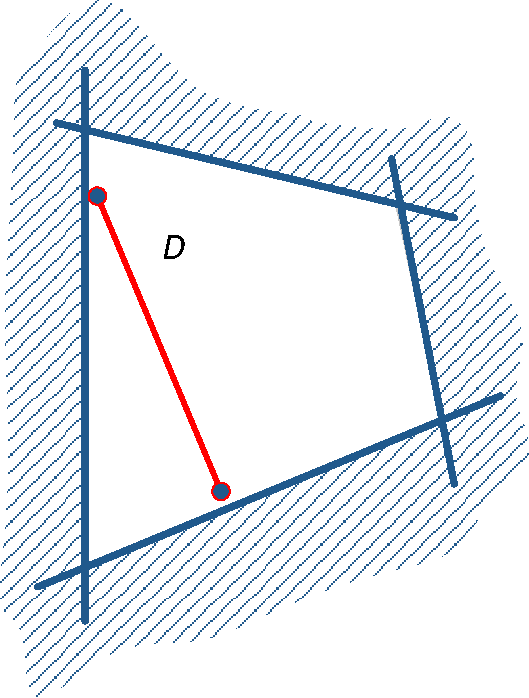
\includegraphics[width=.2\textwidth]{convex} & \hspace*{1cm} & 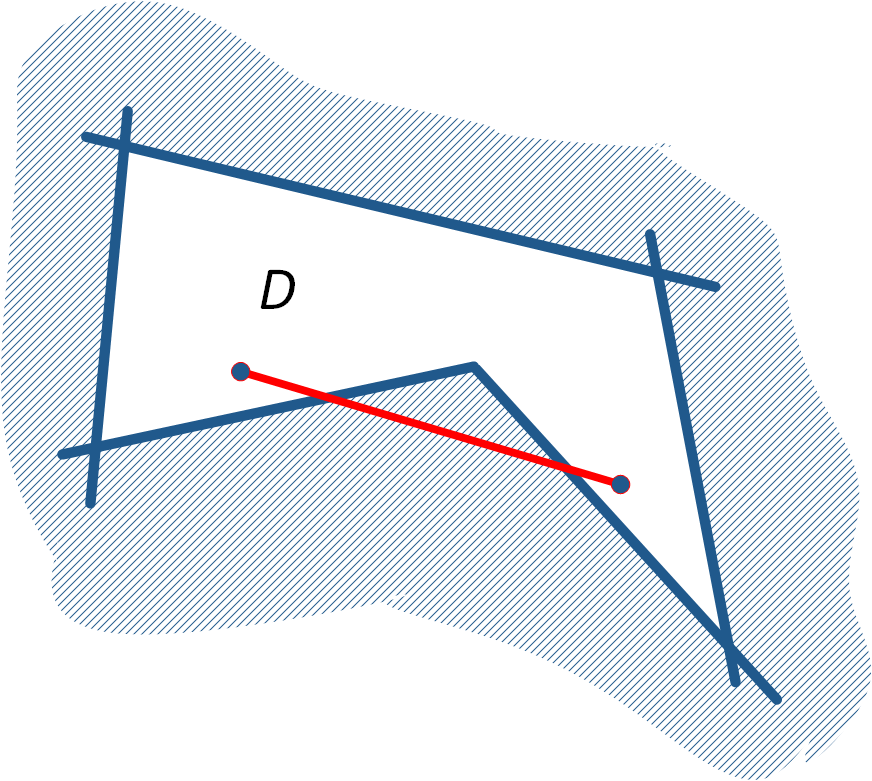
\includegraphics[width=.25\textwidth]{concave} \\
convex & & non-convex / concave
\end{tabular}
\end{center}
\end{frame}

\begin{frame}
  \frametitle{Global Optimum}
\begin{itemize}
\item Convexity gives information about the \emph{curvature}, thus stationary points
\item Constraints of an optimization define the \emph{feasible set} 
\begin{equation*}
D = \left\{ \vecval{x} \in D \,\|\, g(\vecval{x}) \leq 0, h(\vecval{x}) = 0 \right\}
\end{equation*}
which can be either convex or concave
\item Global minima are usually \emph{difficult} to find numerically, except for cases of convex optimization
\end{itemize}

\vspace*{0.4cm}
\textbf{Definition}\\
An optimization problem is \emph{convex} if both the objective function $f$ and its feasible set are \emph{convex}

\vspace*{0.4cm}
\textbf{Theorem} \\
The solution of a \emph{convex optimization} is also its \emph{global solution}
\end{frame}

\section{Wrap-Up}

\begin{frame}
  \frametitle{Summary: Linear Algebra}
{\renewcommand{\arraystretch}{1.5}%
\begin{tabular}{ll}
Dot product & $\vecval{a} \cdot \vecval{b} = \vecval{a}^T \vecval{b}$ \\
Norm & $\norm{\vecval{x}}$ \\
Transpose & $A^T = \left[ a_{ji} \right]_{ij}$ \\
Identity matrix & $I_n = \diag( 1, \ldots, 1 ) \in \R^{n\times n}$ \\
Inverse & $A^{-1} \in R^{n\times n}$ such that $A A^{-1} = I$  \\
Pseudoinverse & $A^+ \in R^{m\times n}$ such that $A A^+ = I$ \\
Determinant & $\det{A}$ \\
Eigenvalue, -vector & $A \vecval{v} = \lambda\vecval{v}$ for $\vecval{v} \neq 0$ \\
Positive definite & $\vecval{x}^T A \vecval{x} > 0$ for $\vecval{x} \neq 0$
\end{tabular}
}
\end{frame}

\begin{frame}
  \frametitle{Summary: Numerical Analysis}
{\renewcommand{\arraystretch}{1.5}%
\begin{tabular}{ll}
Partial derivative & $\frac{\dd f}{\dd x_i}(\vecval{x})$ \\
Finite differences & Numerical approximations to derivatives \\
Gradient & $\nabla f(\vecval{x})$ \\
Hessian & $H(\vecval{x}) = \nabla^2 f(\vecval{x})$ \\
Taylor series & $f(x) = \sum\limits_{n=0}^{\infty}{\frac{f^{(n)}(x_0)}{n!} (x-x_0)^n}$ \\
\end{tabular}
}
\end{frame}

\begin{frame}
  \frametitle{Summary: Optimality Conditions}
\begin{itemize}
\item Local minimum $x^\ast$ if $f(x^\ast) \leq f(x)$ for all $x \in N(x^\ast) \subseteq D$
\item Global minimum if $f(x^\ast) \leq f(x)$ for all $x\in D$
\item Sufficient conditions for a strict local optimizer
\begin{enumerate}
\item $\nabla f(\vecval{x}^\ast) = 0$ (stationarity)
\item $\nabla^2 f(\vecval{x}^\ast)$ is positive definite
\end{enumerate}
\item Convex optimization has a convex objective and a convex feasible set
\item The minimum in convex optimization is always a global minimum
\end{itemize}
\end{frame}

\begin{frame}[fragile]
  \frametitle{Summary: R Commands}
\vfill
%\begin{block}{}
\footnotesize
{\renewcommand{\arraystretch}{1.2}%
\begin{tabular}{ll}
\verb@digitsBase(...)@ & Convert number from base 10 to another base \tabularnewline
\verb@strtoi(...)@ & Convert a number from any base to base 10 \tabularnewline
\%*\% & Dot product, matrix multiplication \tabularnewline
\verb@drop(A)@ & Deletes dimensions in $A$ with only one value \tabularnewline
\verb@t(A)@ & Transpose a matrix $A$ \tabularnewline
\verb@diag(n)@ & Identity matrix of size $n \times n$ \tabularnewline
\verb@solve(A)@, \verb@ginv(A)@ & Inverse or pseudoinverse of a matrix $A$ \tabularnewline
\verb@det(A)@ & Determinant of $A$ if existent \tabularnewline
\verb@eigen(A)@ & Eigenvalues and eigenvectors of a matrix \tabularnewline
\verb@is.positive.definite(A)@, \ldots & Tests if matrix $A$ is positive definite, \ldots \tabularnewline
\verb@D(f, x)@ & Derivative of a function $f$ regarding $x$ \tabularnewline
\verb@eval(f, ...)@ & Evaluates an expression $f$ at a specific point \tabularnewline
\verb@optimHess(...)@ & Approximate to Hessian matrix \tabularnewline
\verb@taylor(...)@, \verb@polyval(...)@ & Taylor approximation\tabularnewline
\end{tabular}
}
%\end{block}
\vfill
\end{frame}

\begin{frame}
  \frametitle{Outlook}
\vfill
\begin{block}{Additional Materials}
Further exercises in homework sheets 3 and 4
\end{block}
\vfill
\begin{block}{Future Exercises}
R will be used to implement optimization algorithms
\end{block}
\vfill
\end{frame}

\end{document}

